\documentclass[11pt]{article}
\usepackage[margin=0.85in]{geometry}
\usepackage[T1]{fontenc}
\usepackage[utf8]{inputenc}
\usepackage{array}
\usepackage[final]{graphicx}
\usepackage{titlesec}
\setkeys{Gin}{draft=false}

\raggedbottom
\setlength{\parskip}{0.35em}
\setlength{\parindent}{0pt}
\renewcommand{\arraystretch}{1.2}
\titlespacing*{\section}{0pt}{0.8em}{0.35em}

\begin{document}

\begin{center}
{\Large \textbf{Group 1 Weather App}}\\
{\large Workflow Diagram}\\
Group 1\\
May 15, 2026
\end{center}
\vspace{0.3em}

\section{Purpose}
This document shows the main workflow for the Group 1 Weather App. The diagram follows a user request from the browser, through the React frontend and Express backend, to the Open-Meteo API. It also shows where the app keeps temporary favorites and search history.

\section{High-Level Workflow Diagram}

\begin{center}
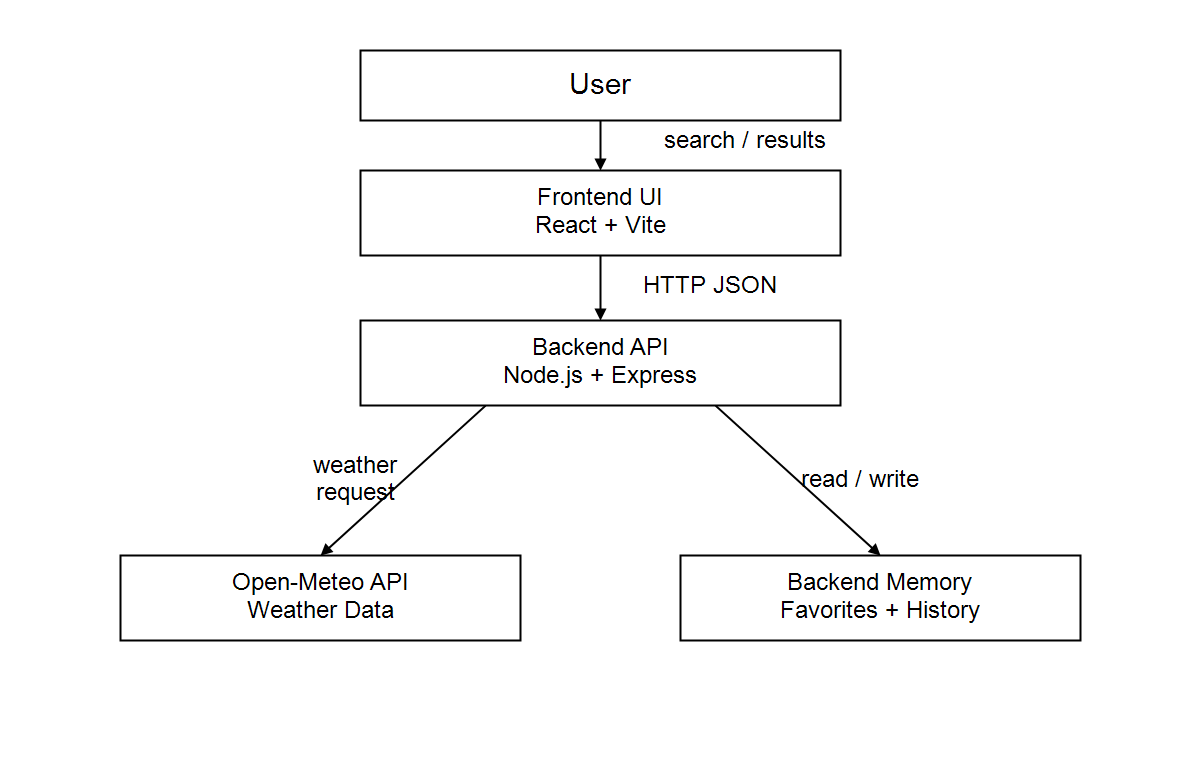
\includegraphics[draft=false,width=0.72\textwidth]{workflow_diagram.png}
\end{center}

\section{Workflow Notes}
\begin{enumerate}
\item The user works through the browser interface.
\item The frontend calls the backend for weather searches, favorites, and history.
\item The backend calls Open-Meteo when it needs live weather data.
\item Search history and favorites are kept in backend memory, so they are temporary.
\item The backend returns JSON, and the frontend uses that data to update the page.
\end{enumerate}

\section{Access and Data Summary}
\begin{tabular}{|p{2.0in}|p{3.8in}|}
\hline
\textbf{Component} & \textbf{Responsibility} \\
\hline
User & Searches for cities, views weather, saves favorites, removes favorites, and views recent searches. \\
\hline
Frontend UI & Sends requests to the backend and displays the returned data. \\
\hline
Backend API & Handles API routes, stores temporary lists, formats weather data, and calls Open-Meteo. \\
\hline
Open-Meteo API & Provides city coordinate lookup and weather forecast data. \\
\hline
In-memory arrays & Hold favorites and recent searches while the backend server is running. \\
\hline
\end{tabular}

\end{document}
